\documentclass[tikz,border=5pt]{standalone}
\usepackage{amsmath,amssymb,fontspec,unicode-math}
\setmainfont{STIXTwoText-Regular.otf}
\setmathfont{STIXTwoMath-Regular.otf}
\usetikzlibrary{positioning,arrows.meta,calc,decorations.pathreplacing}
\begin{document}
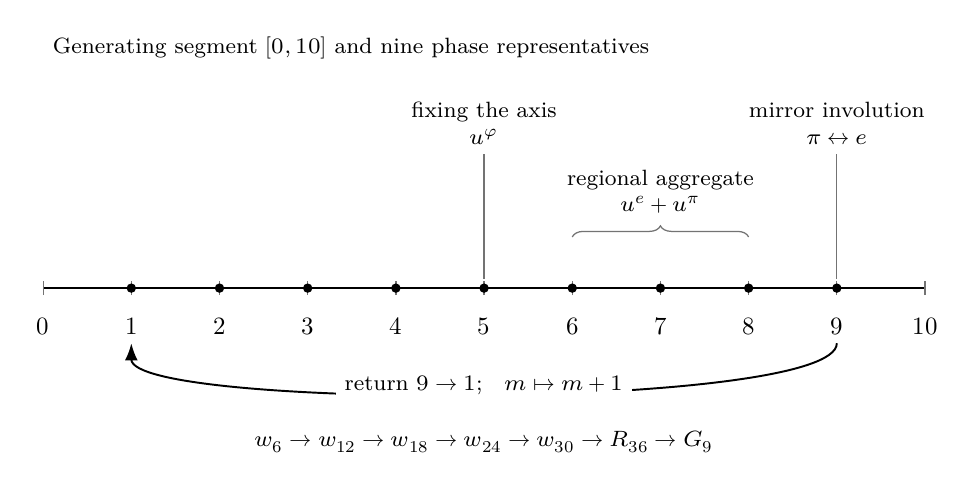
\begin{tikzpicture}[x=1.12cm,y=1cm,font=\small,>=Latex,
  guide/.style={line width=.45pt,black!55}]
 \draw[line width=.8pt] (0,0)--(10,0);
 \foreach \k in {0,...,10}{
  \draw[guide] (\k,-.09)--(\k,.09);
  \node[below=2.5mm] at (\k,0) {$\k$};
 }
 \foreach \k in {1,...,9}{\fill (\k,0) circle (1.7pt);}
 \node[anchor=west,font=\footnotesize] at (0,3.05)
   {Generating segment $[0,10]$ and nine phase representatives};
 \draw[guide] (5,.12)--(5,1.7);
 \node[above,align=center,font=\footnotesize] at (5,1.7)
   {fixing the axis\\$u^\varphi$};
 \draw[decorate,decoration={brace,amplitude=4pt},guide]
   (6,.65)--(8,.65);
 \node[above=5pt,align=center,font=\footnotesize] at (7,.65)
   {regional aggregate\\$u^e+u^\pi$};
 \draw[guide] (9,.12)--(9,1.7);
 \node[above,align=center,font=\footnotesize] at (9,1.7)
   {mirror involution\\$\pi\leftrightarrow e$};
 \draw[->,line width=.7pt] (9,-.7)
   .. controls (9,-1.55) and (1,-1.55) .. (1,-.7);
 \node[fill=white,inner sep=3pt,font=\footnotesize] at (5,-1.23)
   {return $9\to1$;\quad $m\mapsto m+1$};
 \node[font=\footnotesize] at (5,-1.95)
   {$w_6\to w_{12}\to w_{18}\to w_{24}\to w_{30}\to R_{36}\to G_9$};
\end{tikzpicture}
\end{document}

